%\documentclass[letterpaper,twocolumn,10pt]{article}
%\documentclass{sigcomm}
\documentclass{sig-alternate-10pt}
%\documentclass{sig-alternate}

\usepackage{epsfig,endnotes,color,url,paralist, multirow,appendix, graphicx, array}
%\setkeys{Gin}{draft}
\usepackage[lofdepth,lotdepth, farskip=-25pt]{subfig}
\captionsetup[subfloat]{captionskip=-15pt}
\usepackage{float}
%\usepackage{usenix}
\usepackage{times}
\usepackage{xspace}
\usepackage[usenames,dvipsnames,table]{xcolor}
\usepackage{epstopdf}
%\usepackage{citesort}
%\usepackage{etoolbox}
%\patchcmd{\quote}{\rightmargin}{\leftmargin 1em \rightmargin}{}{}
%\newcommand{\simplequote}[1]{\\\noindent{\it``{#1}''}\linebreak[3]}

%%%%%%%%%%%%%%%% Checkmark and Crossmark that match %%%%%%%%%%%%%%%%
\usepackage{pifont}% http://ctan.org/pkg/pifont
\usepackage{amssymb}
\newcommand{\cmark}{\ding{51}}%
\newcommand{\xmark}{\ding{55}}%


%%%%%%%%%%%%%%%%%%%%%%%%%%%%%%%%%%%%%%%%%%%%%%%%%%%%%%%%%%%%%%%%%%%%

\newtheorem{theorem}{Theorem}[section]
\newtheorem{find}[theorem]{Finding}

\newcommand{\paraspace}{\vspace{0.05in}}
\newcommand{\parab}[1]{\paraspace\noindent\textbf{#1} }
\newcommand{\parae}[1]{\paraspace\noindent\emph{#1} }
\newcommand{\parabe}[1]{\paraspace\noindent\textbf\emph{#1} }
\newcommand{\minlan}[1]{{\color{red}[Minlan: #1]}}
\newcommand{\ramesh}[1]{{\color{red}[Ramesh: #1]}}
\newcommand{\rahul}[1]{{\color{red}[Rahul: #1]}}
\newcommand{\Rui}[1]{{\color{blue}[Rui: #1]}}
\newcommand{\navendu}[1]{{\color{blue}[Navendu: #1]}}
\newcommand{\nimbus}{\textsc{nimbus}\xspace}
\newcommand{\delete}[1]{}
% \setlength{\abovecaptionskip}{-0.07in}
% \setlength{\belowcaptionskip}{0in}
% \addtolength{\subfigcapskip}{-25pt}
% \addtolength{\subfigbottomskip}{-50pt}
% \addtolength{\subfigtopskip}{-25pt}
% \addtolength{\subfigcapmargin}{-25pt}
% \addtolength{\subfigcaptopadj }{-25pt}


\newenvironment{encompact}%
{\begin{itemize}%
\setlength{\itemsep}{0pt}%
\setlength{\topsep}{0pt}%
\setlength{\partopsep}{0pt}%
\setlength{\parskip}{0pt}}%
{\end{itemize}}
\setlength{\leftmargini}{9pt}%

 



\begin{document}



\newcommand{\supsym}[1]{\raisebox{4pt}{{\footnotesize #1}}}
\newcommand{\purdue}{\supsym{$\ddag$}}
\newcommand{\msr}{\supsym{$\dag$}}
\newcommand{\usc}{\supsym{$\ast$}}

\twocolumn[%
 \centerline{\Large \bf NIMBUS: Cloud-scale Attack Detection and Mitigation} 
%
 \medskip
%
 \centerline{ 
 Rui Miao\usc \hspace{5mm} 
  Weichen Zhao\usc \hspace{5mm} 
    %Rahul Potharaju\purdue \hspace{5mm}
 Minlan Yu\usc \hspace{5mm}
 %Navendu Jain\msr 
 }
%\medskip
\centerline{ \usc~University of Southern California  \hspace{6mm}
   % \purdue~Purdue University \hspace{6mm}
    %\msr~Microsoft Research 
     }
          
 \bigskip
 ]

%\title{\vspace{-20pt} \Large \bf The Dark Menace: Characterizing Network-based Attacks in the Cloud\vspace{-20pt}}
%%\title{Illuminating the Dark Cloud: \\Characterizing Network-based Attacks in the Cloud}



%\author{
%%Paper \#68, 14 pages
%  Rui Miao\usc \hspace{5mm} 
%   Rahul Potharaju\purdue \hspace{5mm}
% Navendu Jain\msr \hspace{5mm}
% Minlan Yu\usc 
%  \\
%   	\usc~University of Southern California  \hspace{6mm}
%      \purdue~Purdue University \hspace{6mm}
%    \msr~Microsoft Research 
%} 
%  
%\maketitle

%!TEX root = cloudcops.tex
\begin{abstract}
  As the cloud becomes the de-facto platform to deliver online
  services, it is becoming both an attractive target for attackers to
  disrupt hosted services, steal data, and compromise 
  resources to launch attacks on external targets.
  %Yet, very little is known about the prevalence of network-based
  %attacks from and towards cloud infrastructures. 
  In this paper, using three months
  of NetFlow data from a major cloud provider, we present the first
  large-scale characterization of attacks {\em inbound} and {\em outbound} the
  cloud.  We investigate ten types of attacks ranging from network-level DDoS attacks to application-level spam. Our results highlight the complexity, intensity, duration, and distribution of these
  attacks. Our results shed light on the key challenges and solutions for future attack prevention systems in the cloud.
%  Experience with the cloud provider suggests that existing
% defenses are not comprehensive and don't scale to the traffic
% volumes seen in our dataset. From our observation, we provide 
%implications and suggestions on attack detection and mitigation
%at cloud scale.
\end{abstract}

\section{Introduction}
% This paper presents a large-scale field study to characterize
% network-based attacks targeting the cloud
% as well as originating from hosted services/VMs under adversarial
% control.
Cloud services are growing rapidly and their market is expected to reach \$180 billion by 2015~\cite{Gartner}.
%
%Unfortunately, the cloud infrastructure and its hosted
%services are increasingly becoming an important
%target for attacks
Today, large cloud providers host tens of 
thousands of different services, so {\em inbound} attacks targeting the cloud can cause significant, and sometimes spectacular, collateral damage.
A recent survey of datacenter operators indicates that half of them
experienced DDoS attacks, with 94\% of those experiencing regular
attacks~\cite{arborworldwideinfrasecurityreport}. 
%\minlan{cite some arbor report about data center contribute a significant amount of the attacks in the Internet}
Moreover, attackers can abuse hosted services or compromised VMs in the
cloud to launch \emph{outbound} attacks
%in addition to hosting
%malware~\cite{googlesecurityreport,mysqlattack}, stealing confidential
%data~\cite{sonyattack}, 
%disrupting a competitor's service~\cite{darkreading}, and selling
%compromised VMs in the underground
%economy~\cite{caballero2011measuring,stone2011underground}.
%It has been reported that attackers have used cloud VMs 
e.g., to deploy
botnets~\cite{googlesecurityreport}, exploit kits to detect
vulnerabilities~\cite{grier12manufacturing}, send
spam~\cite{kanich11show,tasterchoice}, or launch DoS attacks to other
sites~\cite{booth13cloud}.
In April 2011, an attack on the Sony Playstation network compromising
more than 100 million customer accounts was carried out by a malicious
service hosted on Amazon EC2~\cite{sonyattack}.

According to the recent reports of individual attacks on enterprise and cloud
 networks~\cite{googlesecurityreport,Prolexic}, we highlight several unique features and technical trend
 of attacks in the cloud:
 1) Large-scale. These attacks have 
 the volume up to around 100 Gbps against a single cloud service. 
 2) High diversity of types. The attack types range from network-layer (e.g. SYN flood, UDP flood) to
 application-layer (e.g. HTTP GET, SQL injection) with different characteristics on volume, number of connection, packet header signatures. 
 3) Fast ramp-up rate. The attack traffic ramps up quickly and victimize the target cloud service usually within one minute.
This arises high challenges for attack detection and mitigation in the cloud to meet those requirements.

To detect attacks, cloud operators commonly deploy
commercial hardware boxes at the network, such as Firewalls, IDS, DDoS-protection appliances. 
However, Firewalls and IDS usually fail under high attack load. Even the specialized DDoS-protection appliances
(which focuses on volumetric attacks) is sometimes overwhelmed by the volume of attack
traffic seen by the cloud provider. Moreover, the DDoS-protection appliances has high monetary cost and inflexible progammability with third party software. Other software-based middleboxes (e.g. load balancers, OpenNF) can be specified to aid attack detection but they also cannot handle such high traffic load and it is still challenging to have quick detection relative to attack ramp-up rate. 
%
Prolexic~\cite{Prolexic} provides high-capacity private scrubbing networks but it also relies on fast and accurate attack detection. Further, it requires the traffic to be re-routed, which is not feasible for private tenant traffic in the cloud.
%
Google adopts an approach of absorbing DDoS bursts by killing low-priority jobs and pooling available servers. However, it is impossible to kill tenant instances in a multi-tenant cloud. 
%
None of these above systems provides comprehensive
coverage of the large attack diversity in the cloud. 

In this paper, we propose a new paradigm of  
{\em detection-as-a-service} and {\em mitigation-as-a-service}
that leverages commodity VMs for attack detection. 
%somewhat counter-intuitive solution: using
Our approach, instantiated in a service called \nimbus, combines the
elasticity of cloud computing resources 
with the kinds of programmability seen in software-defined networks
(SDN).
%
It allows us to scale resource usage with traffic demands, flexibility
to handle attack diversity, and resilience against volumetric attacks
designed to subvert the detection infrastructure.
%
\nimbus's central controller directs different traffic aggregates to
different VMs, each of which detects attacks destined to different
sets of cloud services.
%
Each VM can be easily programmed to detect the wide variety of attacks
discussed above, and when a VM is close to resource exhaustion, the
controller can divert some of its traffic to other, possibly newly
instantiated, VMs.
%
There are several key challenges in designing and implementing
\nimbus: including auto-scaling VMs to minimize traffic
redistributions, devising appropriate interfaces between the
controller and the VMs, and determining an efficient yet clean
functional separation between user and kernel-space processing for
traffic.
%
Our prototype built using servers with 10G links shows that \nimbus
can quickly scale-out virtual machines to analyze traffic at line
speed while providing reasonable accuracy for attack detection.




 
%\input{overview}
%\input{traffic}
%\input{characteristics}
%\input{source}
\section{Background and Motivation}

In this section we first motivate the need to detect and mitigation
network-based attacks in the cloud and then discuss the limitation of current 
approaches.

\subsection{Network-Based Attacks in the Cloud.}
The cloud network we study comprises multiple geographically
replicated datacenters connected to each other and to the Internet via
edge and core routers (collectively called border routers).
%
The provider hosts multiple services and each hosted service is
assigned a public virtual IP (VIP) address; we use
the terms VIP and service interchangeably.
%
User requests are typically load balanced across a pool of servers
that are assigned direct IP (DIP) addresses for intra-datacenter
routing. 
%\ramesh{Can a service be hosted on multiple sites? Does it have one VIP?}
%
Incoming traffic first traverses the border routers, then security
appliances like firewalls, DDoS protection appliances and intrusion detection systems, before
hitting the load balancers that distribute traffic across service DIPs.
%
In this paper, we study network-based attacks on cloud infrastructure
(henceforth, \emph{cloud attacks} or simply attacks).

Two aspects of cloud infrastructure make it important to study cloud
attacks.
%
First, compared to enterprise-hosted services, cloud services have
much greater diversity and scale; the cloud provider we study hosts
more than 10,000 services ranging from web storefronts, media streaming,
mobile apps, storage and backup to large online marketplaces. 
%
Unfortunately, this also makes the cloud a %attractive %natural 
target for attackers; a single, well-executed attack can cause more direct
and collateral damage than individual attacks on enterprise-hosted services.
%
While such a large service diversity allows observing 
a wide variety of \emph{inbound} attacks, it 
also makes it hard to distinguish attacks from legitimate traffic 
as these services likely generate {\em all possible} traffic patterns in normal operation.
%
%\ramesh{Navendu, please check and elaborate on this point.}

Second, attackers can abuse the cloud resources to launch \emph{outbound} attacks.
For instance, they can launch brute-force attacks (e.g., password guessing) to 
compromise vulnerable VMs 
%Further, poor security practices and lack of control on third-party tenants may expose
%vulnerabilities which attackers would be likely to compromise and exploit. 
%The VMs running services on the cloud can be compromised using automated, vulnerable VMs 
and gain bot-like control of the infected ones.
%
These compromised VMs may be used for a variety of adversarial purposes such as
YouTube click fraud, BitTorrent hosting, illegal Bitcoin
mining, send SPAM, propagate malware, or launch bandwidth-flooding DoS attacks
(cloud providers typically cap outgoing bandwidth per VM, but not in aggregate across a tenant.).

\subsection{Limitations of current approaches.}
%
While many of these approaches are relevant to cloud defense (such as
end-host filtering, and hypervisor controls), commercial DDoS-protection
 appliances are commonly deployed for dedicated attack detection and mitigation. 
 %
However, from the observation of recent attacks, we argue that those commercial hardware appliances 
are inadequate for attacks in cloud scale, for
three reasons.

% While current commercial security appliances are effective at safeguarding a variety of attacks,
% they have three key limitations for deployment at cloud scale.

\parae{High Cost.} These hardware boxes introduce unfavorable cost
vs. capacity tradeoffs. In particular, they cost hundreds of thousands
up to a few million dollars per box, but can {\em only} handle up to
tens of gigabytes of traffic and risk failure under both network-layer
and application-layer DDoS attacks.
%In a 2011 survey, 36\% and 42\% of the respondents indicated failure of a firewall due to  at the application layer and network layer, respectively
%~\cite{2011 ADC Security Survey Global Findings, http://goo.gl/A3b2Q}.
~\cite{ADC}

Thus, to handle
traffic volume at cloud scale and increasingly high-volume DoS attacks 
(e.g., 300 Gbps+~\cite{Q4report}), this approach would incur significant costs. Further, these devices
need to be deployed in a redundant manner further increasing procurement and 
operational costs. 
%for fault tolerance. 

\parae{Inflexibility.} Since these devices run proprietary software, they limit
how operators can configure them to handle the increasing diversity of attacks today. 
Given lack of rich programmable interfaces, 
operators are forced to specify and manage a large number of policies themselves  
for controlling traffic e.g., set thresholds for different protocols, ports, cluster, VIPs 
at different time granularities. Further, 
they limit effectiveness against increasingly 
sophisticated attacks.
% such as zero-day attacks. %detection and patching.
Finally, these third-party devices may not be kept up to date with OS, firmware and builds which risks reducing their effectiveness against attacks. 
%However, today's hardware appliances can only support a limited number of policies (< 1K) and a limited number of mitigation rules (<50). \minlan{why?}

\parae{Risk collateral damage.} Since many attacks can ramp up
in 10s of seconds to a few minutes, a
relatively high detection latency risks overloading the target VMs as
well as the shared cloud infrastructure e.g., firewalls, load
balancers and core links, which may cause collateral damage to
co-hosted tenants.  Similarly, if we cannot revert fast
enough when the attack subsides, we may mistakenly block legitimate
traffic. Given that many security solutions apply traffic
profiling and smoothing techniques to reduce false positives for
attack detection~\cite{peakflow}, they may not be able to act quickly
enough to avoid collateral damage.

\subsection{Detection/mitigation-as-a-service}
To overcome some of these limitations, we argue that we need to
re-think attack detection in the context of clouds.  To this end, we
describe the architecture of \nimbus, a scale-out VM-based service for
detecting and mitigating to network-based attacks in the cloud.  In contrast
to expensive hardware appliances, our key idea is to leverage the core
principles in cloud computing (elastic scaling of resources on demand)
and software-defined networks (programmability of multiple network
layers) to introduce a new paradigm of {\em detection-as-a-service}
and {\em mitigation-as-a-service}.  We first present the requirements
based on our measurement study and then describe its design and
implementation.

\parab{1.} Scaling to match datacenter traffic capacity at the order of hundreds of gigabits per second. 
The service should auto-scale to enable agility and cost-effectiveness.  

\parab{2.} Programmability to handle new and diverse types of network-based attacks, and flexibility to    
allow tenants/operators to configure policies %and roll out updates %in an attack-specific and traffic-based patterns. %schemes that are 
specific to the traffic patterns and attack characteristics.

\parab{3.} Fast and accurate detection and mitigation for attacks that ramp-up within one minute; 
once the attack subsides, we should revert the mitigation to avoid blocking legitimate traffic. 

\parab{4.} Robustness to prevent sophisticated attacks from a wise adversary, who knows our system well and want to victimize either the detection service or individual cloud service. 




\section{design}

\begin{figure}[t!]
 \centering
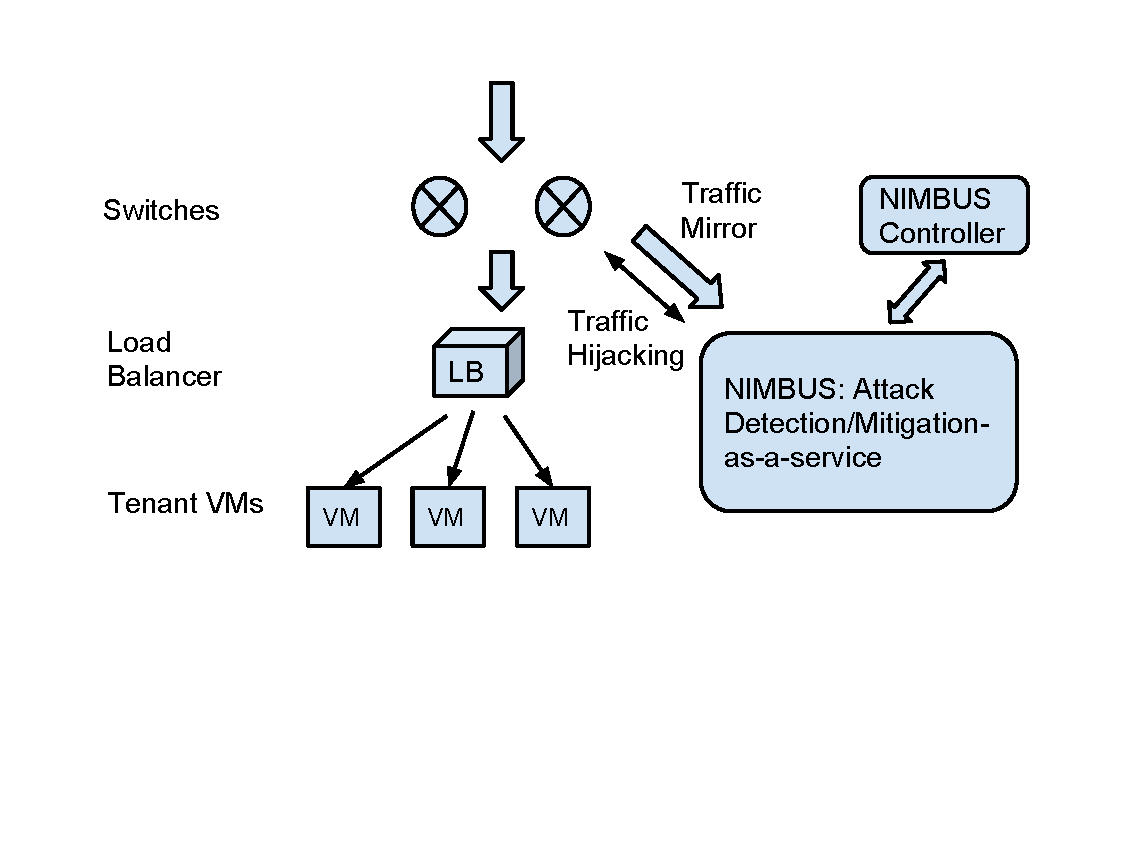
\includegraphics[width=\linewidth]{figs/scope.pdf}
\vspace{-0.82in}
\caption{\small Network scope of \nimbus deployment}
\vspace{-0.0in}
\label{fig:scope}
\end{figure}

\begin{figure}[t!]
 \centering
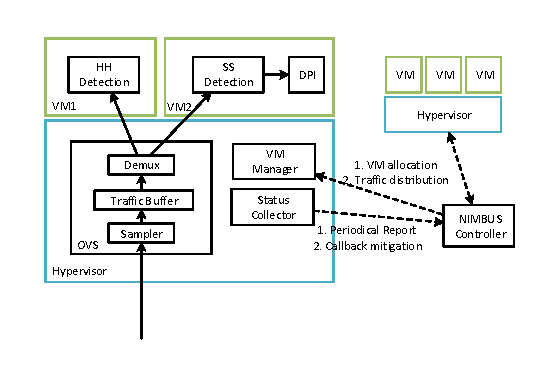
\includegraphics[width=\linewidth]{figs/arch.pdf}
\vspace{-0.22in}
\caption{\small \nimbus Architecture}
\vspace{-0.2in}
\label{fig:design}
\end{figure}


\nimbus can be deployed as either an in-band or an out-of-band
solution. The in-band solution requires faster scale-out to avoid affecting the data path and to ensure packet forwarding at line speed.
However, our prototype investigate the outband solution to avoid taking resources from the critical infrastructure (e.g., switches, software load balancers). 
As shown in Figure ~\ref{fig:scope}, it requires the extra overhead of duplicating (e.g., port mirroring) the traffic to the detection and mitigation service. Further, as part of mitigation, \nimbus can also hijack a portion of traffic for scrubbing and send traffic back to network after dropping all attack traffic.

%\nimbus can be used for both inbound and outbound attacks. \minlan{anything more to say?}

%While \nimbus was designed to overcome limitations in commercial
%appliances, these can complement \nimbus nicely.  For example, we can
%leverage a scrubbing layer in switches to reduce the traffic to our
%service or use \nimbus to decide when to forward packets to
%hardware-based anomaly detection boxes for deep packet inspection.

We have designed \nimbus as a distributed architecture
(Figure~\ref{fig:design}) 
using an SDN-inspired framework, 
comprising a set of VM instances that analyze traffic for attack detection  
(called \emph{VMSentries}) and an \emph{auto-scale controller}
that (a) does scale-out/in of VM instances to avoid overloading,
(b) manages routing to traffic flows to them, and 
%(c) traffic sampling modules and 
(c) dynamically instantiates anomaly detector and mitigation modules on them.
%To enable applications and operators to flexibly specify their sampling, attack detection and mitigation strategies, 
%\nimbus exposes these functionalities through a RESTful API shown in Table~\ref{tab:autoscale-apidesign}. 

\parab{VMSentry.} The VMSentry is a pool of VMs instantiated on-demand for attack detection and mitigation. 
The role of a VMSentry is to passively collect ongoing traffic (e.g., via sampling), 
analyze it via detection modules, and prevent unauthorized traffic as configured by the SDN controller. 
The traffic is sampled in hypervisor and delivered to specific VM for analysis.
For each VMSentry, the control application 
would instantiate 
(1) a detector (e.g., heavy-hitter for TCP SYN/UDP floods, super-spreader for DNS reflection),
(2) configure the sampler in hypervisor for the new VM (e.g., sampling rate).
  %(2) attach a sampler (e.g., flow-based, packet-based, sample-and-hold) and set its configurable sampling rate, 
%(3) provide a callback URI, and 
(3) then install it on that VM. 
When the detector instances detect an on-going attack, they invoke a callback to controller. The controller can then decide to 
specify a mitigation strategy in an application-specific manner. 
For instance, it can set up rules for access control, rate-limit or redirect 
anomalous traffic (not the copy) to \nimbus devices for scrubbing or an in-depth analysis. 
Setting up mitigator instances is similar to that of detectors with a specific mitigator action (e.g., redirect, scrub, mirror, allow, deny) .
%and %optionally 
%specify the flow (either through a standard 5-tuple or $<$VIP, protocol$>$ pair) along with a callback URI.

Our implementation of \nimbus 
separates mechanism from policy by partitioning VMSentry functionalities between the hypervisorl and VM: 
packet sampling is done at the hypervisor for performance and efficiency, 
%hypervisor layer for performance and efficiency, 
%(reduce the number of packets sent to the user space) 
and the 
detection and mitigation policies reside in the VM's user space to ensure flexibility and adaption at run-time.
This separation allows 
multi-stage attack detection and mitigation e.g.,  traffic from source IPs sending a TCP SYN attack can be forwarded for deep packet inspection.
The intuition behind co-locating detectors and mitigators on the same VM instance 
is that it reduces the critical overheads of  
traffic redirection, which can be significant~\cite{Sylvia2011}, and leverages the caches to store the packet content. Further, this approach  
avoids the controller overheads 
of managing different types of VMSentries. 
%that gets called when the mitigator detects the termination of an on-going attack. 

Given limited computing and memory capacity in VM instances, a key question is what granularity to use to uniquely identify 
and specify actions on anomalous flows. %Specifically, 
While using the five-tuple flow identifier allows flexibility to specify detection and mitigation at a fine granularity,  
it risks high resource overheads, 
missing attacks at the aggregate level (e.g., VIP) or treating correlated attacks as independent ones. 
In the cloud setup, since traffic flows can be logically partitioned by VIPs, \nimbus addresses flows using $<$VIP, protocol$>$ pairs. This allows us to 
(a) efficiently manage state for a large number of flows at each VMSentry,
and (b) design customized attack detection solutions for individual VIPs;
we leave the investigation of flow identifiers at finer granularities for future work.
Note that the traffic flows for a $<$VIP, protocol$>$ pair can
be spread across VM instances 
similar in spirit to SLB~\cite{Patel13}. 
%akin to SLB~\cite{Patel13}.  
%\navendu{DO YOU MEAN "we allocate one  $<$VIP, protocol$>$" OR "detector+mitigator" to the same VM.} \minlan{one  $<$VIP, protocol$>$} \navendu{minlan: I'm not clear how to weave in this argument (vip,prot) split across vms like in slb (using ECMP; all SLBs have identical VIP to DIP mapping) or keep to a single one 
%\navendu{Rui: anything else to add?} 
	
% \delete{
% 	As our measurement results show, different protocols are vulnerable for different types of attacks. For example, RDP traffic are usually under spread-based attacks while TCP traffic are more vulnerable to volume based attacks. 
% The management decisions on VIP and protocol fields only can guarantee the scalability of our system. (Note that SLB also made load balancing decisions on VIPs to ensure scalability.)
% However, we choose not to use finer granularities (e.g., five tuple flows) to reduce the overhead of managing the system. 

% There are two ways of using the VMs when each $<$VIP, protocol$>$ needs a pipeline of detection and mitigation solutions. First, we can use each VM to run one function (e.g., heavy hitter detection) but then redirect traffic to different VMs for different functions. Second, we can use one VM to perform all the attack detection/mitigation solutions for the same $<$VIP, protocol$>$. 
% }


\parab{SDN auto-scale controller.} 
The controller collects the load information across instances every 
measurement interval. 
If needed, it computes a new allocation of traffic distribution across existing VMs and
scale-out/in VM instances. Finally, it installs routing rules to redirect the traffic. 


%\parae{Traffic splitting to VMs:} 
In the cloud environment, the traffic patterns destined to a VMSentry may quickly increase due to higher traffic rate of 
existing flows (e.g., volume-based attacks) or setup of new flows (e.g., due to tenant deployment). Thus, a 
key requirement is to avoid overload of VMSentry instances as it risks impacting accuracy and effectiveness of attack detection and mitigation. 
To address this issue, the controller monitors load at each instance
and dynamically re-allocates traffic across the existing and possibly newly-instantiated VMs. 
To implement this functionality, however,  
we need to make three design decisions: 
(1) What metric to use to measure load? 
(2) How to redistribute traffic across instances? and 
(3) Do we need to transfer flow state from an overloaded instance to a new/existing one? 

First, we choose to use CPU as the VM load metric because our experiments show that CPU utilization is strongly correlated to traffic rate. 
%he packet sampling at the kernel and the packet inspection at the user space are two potential bottlenecks and both are bottlenecked by their CPU usage. We can also extend this to other metrics such as memory and bandwidth usage. 
We model CPU usage as a function of the traffic volume for different anomaly detection/mitigation algorithms to set the maximum and minimum load threshold. 

Second, to redistribute traffic, we formulate a bin-packing problem which takes the top-k $<$VIP, protocol$>$ tuples by traffic rate as input from the overloaded
VMs and uses the first-fit decreasing algorithm that allocates traffic to the 
other VMs while minimizing the migrated traffic. If the problem is infeasible,
it allocates new VMSentry instances so that no instance is overloaded. Similarly, for scale-in, all VMs whose load falls below the minimum threshold become 
candidates for standby or being shut down. The VMs selected to be taken out of operation stop accepting new flows and transition to inactive state once incoming traffic ceases. Note that other traffic redistribution and auto-scaling approaches can be applied in our framework.   
We observe that many attack detection/mitigations tasks are state independent. For example, to detect the heavy hitters of traffic to a VIP, we typically need to keep track of the traffic volumes only in the 
most recent intervals. This simplifies traffic redistribution as we do not need to transfer potentially large measurement state of transitioned flows.
For those measurement tasks that do need state transitions, we can 
add a constraint for the traffic distribution algorithm 
to avoid moving their traffic. 

Third, to redistribute traffic, the controller changes routing entries at the upstream switches/routers to redirect traffic. 
Finally, to quickly transition the service to a stable state during churn, \nimbus maintains a standby resource pool of VMs which
are in active mode and can take the load immediately.
%hich have much shorter restart times compared to loading and deploying new VM images from disk;
We show the efficacy of this approach in next section.




\section{evaluate}

\section{Discussion}

\parab{Robust to wise adversary.}
A wise adversary may be aware of our detection and mitigation system and generate sophisticated attacks to a) evade our \nimbus system; b) reduce the effectiveness of \nimbus system.
%
For example, the wise adversary may generate attack burst in a very short amount of time and repeat it periodically but with a relatively low average throughput. 
%
\nimbus may highly likely miss this attack from the use of traffic sampling. 
%
Another example, the wise adversary may become aware of the stage of mitigation. So he can subside the attack when \nimbus is scaled-up and launch it again when the system is about to scale-back. Doing so will cause fluctuation and decreasing efficiency in our system.
%
How to design a robust system to defense such a wise adversary is a challenge problem.

\parab{Mitigation-as-a-service.}
Once an attack being identified, the system needs to provide a set of functionalities to mitigate attacks.
%
Since the system can track the traffic changes, it can potentially identify the begin of an attack. 
%
For example, we can identify and mitigate an attack when the traffic starts to ramp-up and, as a result, minimize its damage to the target service. 
%
In this sense, we need to investigate when to start and stop the mitigation, which flow to mitigate so we achieve both effectiveness and low collateral damage to legitimate traffic, 
and how to adjust detection accuracy for fast attack detection but with low false positive. 
%
In general, we need to consider the balance of resource usage of detecting and mitigating attacks, detection accuracy, and collateral damage to legitimate traffic.


%\input{correlation}
%\input{validation}
%\input{implication}
\section{Related Work \label{sec:related}}

%Our work is inspired by related work in attack detection as discussed below.

%\parab{Attack detection techniques and systems:}
%
There have many proposals for efficient measurement and detection of
attacks
using specialized network hardware~\cite{estan2003new, minimalist, csamp}.
Sekar et al.~\cite{sekar2006lads} develop a triggered, multi-stage DDoS detection system 
for a large ISP to identify customers under attack. 
Kandula et al.~\cite{kandula2005botz} propose improvements to 
CAPTCHA-based defenses to 
identify attackers that keep sending wrong solutions at a high-rate. 
 Ranjan et al.~\cite{ranjan2006ddos} propose a session scheduling algorithm to detect DoS attacks. 
Lo et al.~\cite{lo2010cooperative} propose a cooperative IDS approach  
where attack alerts are exchanged between different regions in a cloud network. 
Our work explores a complementary direction of integrating elasticity 
using commodity VMs and programmability in SDNs to enable detection
and mitigation as a service.
% 
%-based framework that is flexible for operators to plug in different measurement solutions.
%
In comparison to prior  measurement systems~\cite{csamp, opensketch,
  measurement:techrep} which allocate fixed amount of resources to different
measurement tasks, our programming abstractions enable 
dynamically adapting resource usage in proportion to traffic. 
Auto-scaling has also been used 
%is commonly used in cloud computing to handle dynamic workload
%patterns for inhas also been used in other efforts 
to support load balancing~\cite{Patel13} and resource allocation for
job execution~\cite{tide, autoscale}.
% We design an autoscale system for attack detection by leveraging the elasticity of VMs in the cloud.

% There are three attacker detection approaches: misuse detection, anomaly detection, and specification-based detection~\cite{mirkovic2004taxonomy}. 
% Honeypots are usually an effective detection tool against many DoS attack instances~\cite{spitzner2003honeypots}. For instance, in shadow honeypots, false alarms are reduced by re-routing suspected requests transparently to instrumented servers to detect attacker attempts to exploit vulnerabilities~\cite{anagnostakis2005detecting}. 
% Estan et al.~\cite{estan2003new} propose an elegant algorithm to detect \textit{heavy-hitter} network flows with low memory requirements to suit in-router implementations. Their sample-and-hold
% technique is proposed for network-level detection and requires an operator-specified threshold to identify heavy-hitters. 
% %To detect flows that deviate from pre-defined specifications, Chuah et al.~\cite{chuah2003dcap} proposed an $\sqrt{N}$ distributed algorithm. 
% Kandula et al.~\cite{kandula2005botz} improve CAPTCHA-based defenses by detecting attackers that keep sending wrong solutions at a high-rate. 
% Ranjan et al.~\cite{ranjan2006ddos} enumerate a set of abnormal request behaviors that DDoS attackers use and propose a session scheduling algorithm based on a per-session based suspicion level. The paper~\cite{feamster-2006-sigcomm} leverages network traffic patterns to detect spams.
% Our work is not novel in attack detection solutions, but instead combines existing methods that fit cloud attack detection by leveraging NetFlow data (for anomaly detection), botnet locations (for specification-based detection), and honeypot data (for misuse detection). 


%The application of intrusion detection systems (IDSes) in cloud environments is a research field
%that is gaining interest~\cite{vieira2010intrusion,kenny2005towards,roschke2009intrusion} due to the increasing prominence of cloud computing services. Leu et al.~\cite{leu2005integrating} present a solution based on analyzing data from a grid's network although they cannot detect grid-specific attacks. Feng et al.~\cite{feng2006ghids} integrate a host-based IDS into a grid environment, providing protection against typical operating system attacks, but not the ones that might target middleware vulnerabilities. Lo et al.~\cite{lo2010cooperative} propose a cooperative intrusion detection system for cloud computing network to reduce the impact of a DoS attack where cloud computing regions under attack exchange alert messages to learn from the experience of others. 
%In addition, many industry providers collaborate in sharing data on attacks and vulnerabilities to prevent their spread and develop mitigation techniques~\cite{csc}. 
%Google maintains a web security site listing up to 10K infected %malware and phishing 
%sites and found that most malware-ridden sites are legitimate ones~\cite{googlesecurityreport}.


%how long it takes compromised sites to clean up~\cite{}.
%http://technet.microsoft.com/en-us/library/cc959354.aspx

% \parab{Attack mitigation methods:}
% There have also been a large amount of work on attack mitigations.
% Blasklist is the most common strategy and many papers (DOMINO) have evaluated the scale and temporal effect of blacklist.
% "DDoS Defense by Offense sigcomm 06" the victim service encourages good clients to inflate their traffic so as to crowd out attack traffic.


%  For example, 
% Kargl et al.~\cite{kargl2001protecting} propose using class-based queuing and traffic monitoring to protect web servers from DDoS attacks. 
% %Jin et al.~\cite{jin2003hop} proposed the hop-count filter to detect and block packets with spoofed source addresses. 
% Yaar et al.~\cite{yaar2004siff} present a capability-based scheme where attack victims recover by revoking access from detected attackers. 
% To recover from spoofing attacks, traceback mechanisms (e.g., ~\cite{savage2000practical}, ~\cite{bellovin2003icmp}) have been proposed. 
% % Vulimiri et al.~\cite{vulimiri2012well}  quantify the protection that congestion pricing affords against DDoS attacks, even for powerful attackers that can control their packets' routes and show that their scheme is provably superior to fair queuing in attack resilience. 
% Mahajan et al.~\cite{mahajan2002controlling} propose mechanisms for detecting and controlling high bandwidth aggregates
% %Their design involves both local mechanisms for detecting and controlling an aggregate 
% at a single router, and a cooperative pushback
% mechanism in which a router can ask upstream routers to control an aggregate. 
% % \delete{
% % Another approach in the in-network filtering line of work is the scheme introduced by Max-min fair throttling~\cite{yau2005defending} in which the basic idea is to install a router throttle at selected upstream routers that allow routers to proactively regulate packet rates to moderate levels.
% % }
% % Other techniques such as using authentication inside the network will also help defend against DDoS attacks e.g., IPSec~\cite{kent1998security}. For instance, Gouda et al.~\cite{gouda2002hop} propose a framework for providing hop integrity in computer networks. 
% Our work provides insights on the requirements of attack mitigation solutions for network-based attacks in the cloud.



%http://research.zscaler.com/2012/01/popularity-of-exploit-kits-leading-to.html
%http://cseweb.ucsd.edu/~klevchen/pkvls-imc12.pdf
%http://cseweb.ucsd.edu/~klevchen/lpcefghkklmwpvs-oakland11.pdf
%http://cseweb.ucsd.edu/~klevchen/kcmgwmlvs-cset11.pdf
%http://cseweb.ucsd.edu/~klevchen/gbccdlmmnpprrrtpsv-ccs12.pdf
%http://technet.microsoft.com/en-us/library/cc959354.aspx
%http://www.networkcomputing.com/security/ddos-attacks-getting-bigger-report-finds/240159255
%http://cseweb.ucsd.edu/~savage/papers/CCS12Exploit.pdf
%http://twimgs.com/darkreading/cloudsecurity/S6870413_DR_Cybercriminals.pdf
%%% Local Variables: 
%%% mode: latex
%%% TeX-master: "cloudcops"
%%% End: 

%\section{Discussion}

\parab{Robust to wise adversary.}
A wise adversary may be aware of our detection and mitigation system and generate sophisticated attacks to a) evade our \nimbus system; b) reduce the effectiveness of \nimbus system.
%
For example, the wise adversary may generate attack burst in a very short amount of time and repeat it periodically but with a relatively low average throughput. 
%
\nimbus may highly likely miss this attack from the use of traffic sampling. 
%
Another example, the wise adversary may become aware of the stage of mitigation. So he can subside the attack when \nimbus is scaled-up and launch it again when the system is about to scale-back. Doing so will cause fluctuation and decreasing efficiency in our system.
%
How to design a robust system to defense such a wise adversary is a challenge problem.

\parab{Mitigation-as-a-service.}
Once an attack being identified, the system needs to provide a set of functionalities to mitigate attacks.
%
Since the system can track the traffic changes, it can potentially identify the begin of an attack. 
%
For example, we can identify and mitigate an attack when the traffic starts to ramp-up and, as a result, minimize its damage to the target service. 
%
In this sense, we need to investigate when to start and stop the mitigation, which flow to mitigate so we achieve both effectiveness and low collateral damage to legitimate traffic, 
and how to adjust detection accuracy for fast attack detection but with low false positive. 
%
In general, we need to consider the balance of resource usage of detecting and mitigating attacks, detection accuracy, and collateral damage to legitimate traffic.


%\input{conclusion}

%\newpage
{\bibliographystyle{abbrv}
\bibliography{reference}}

\end{document}
